\begin{figure*}[t]
  \begin{center}
  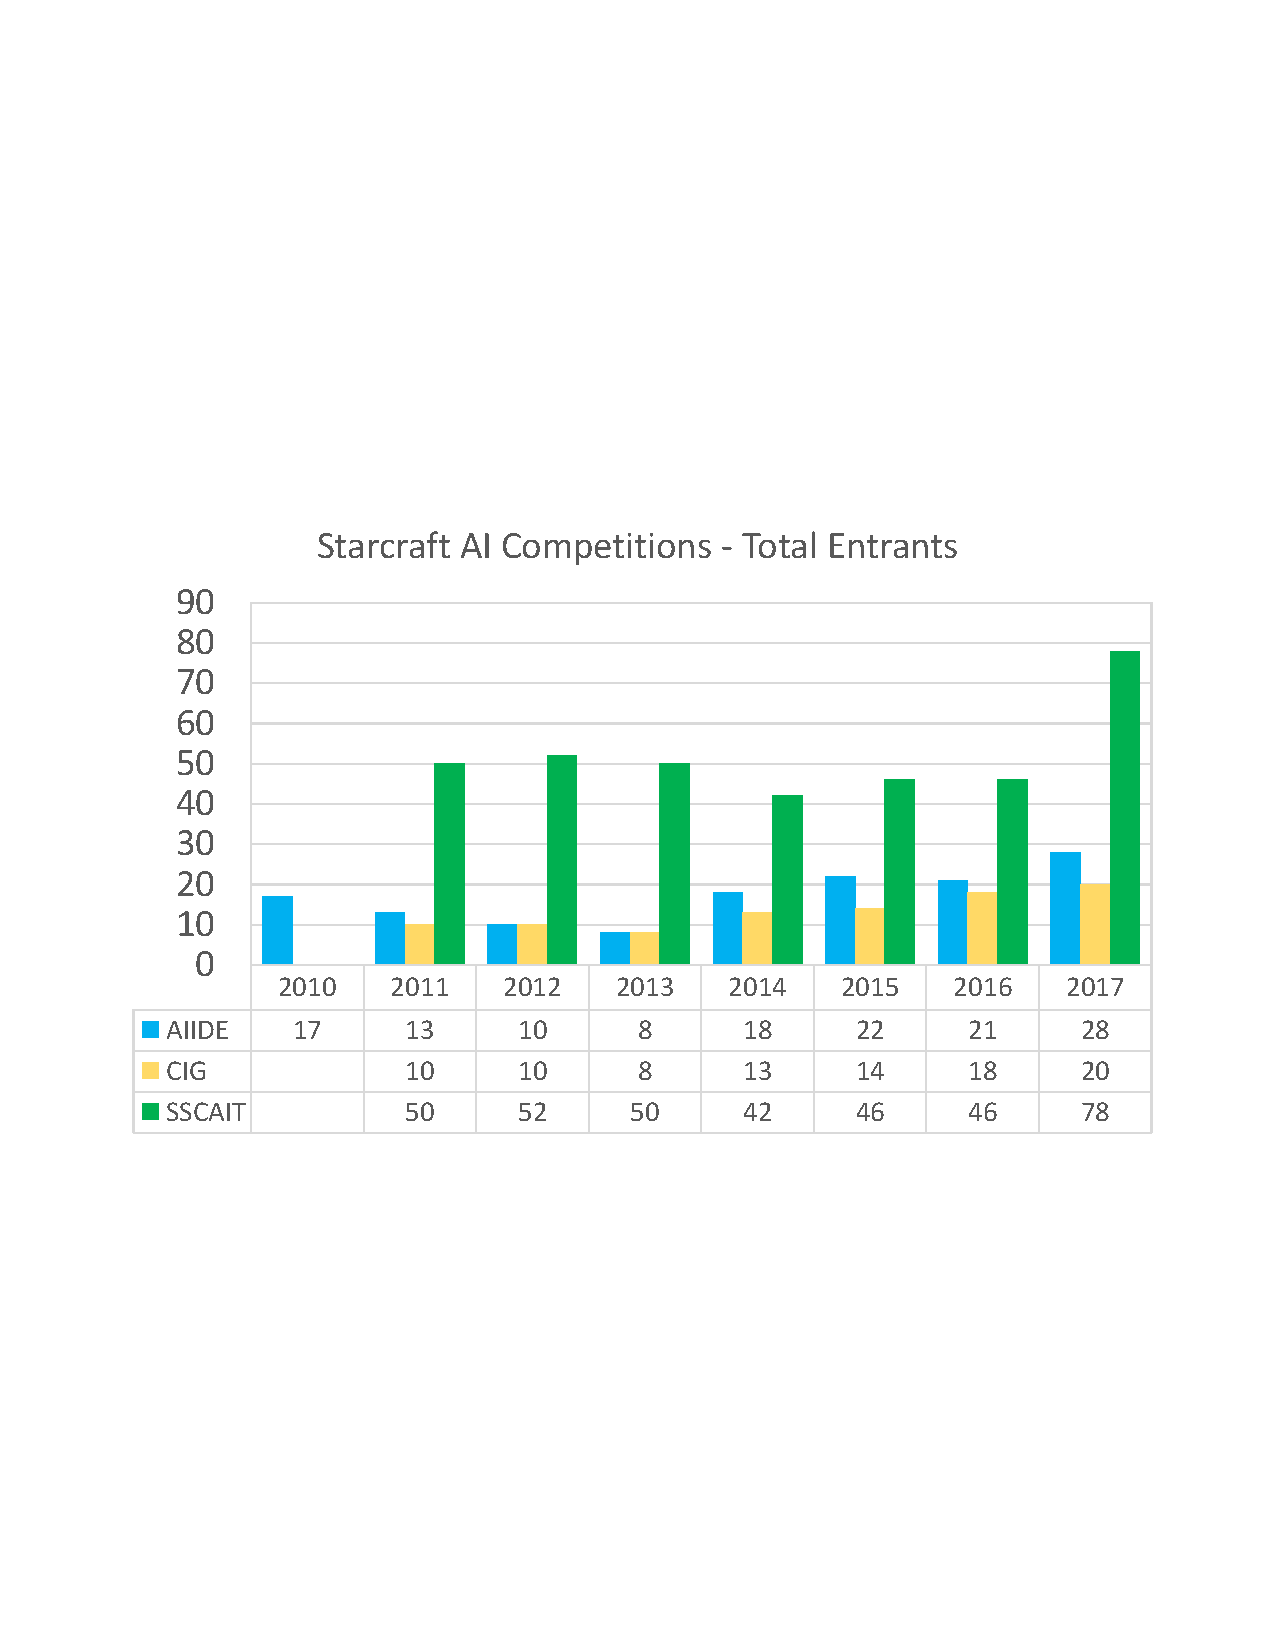
\includegraphics[width=1.05\columnwidth]{fig/Entrants}
	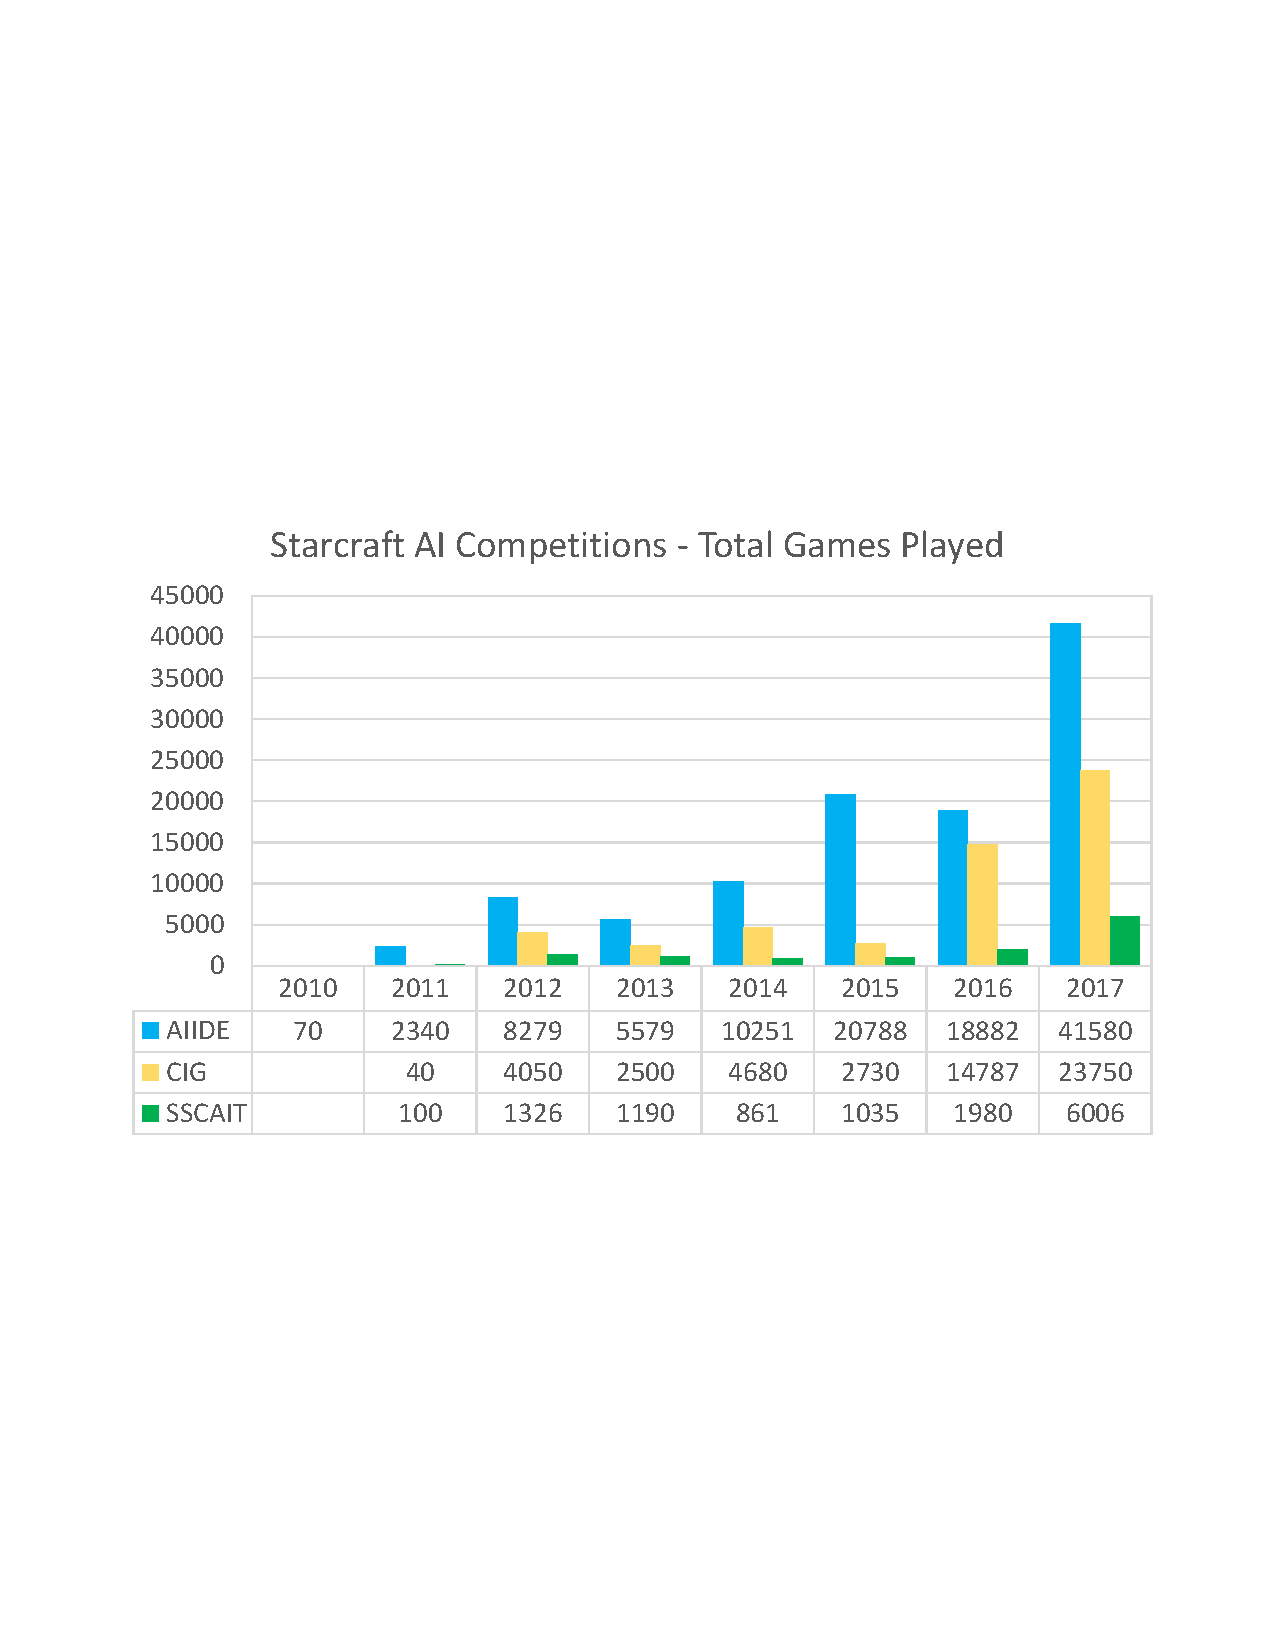
\includegraphics[width=1.05\columnwidth]{fig/GamesPlayed}
%  \vspace{-0.2cm}  
  \caption{Statistics for each of the 3 major annual StarCraft AI Competitions: AIIDE, CIG, and SSCAIT, since the first competition in 2010. Shown on the left is the number of total entrants for each competition, and on the right are the total number of games played in each competition.  }
  \label{fig:comps}
  \end{center}
  \vspace{-0.5cm}
\end{figure*}

\section{Current StarCraft Bots}\label{secBots}

Over the years, StarCraft AI competitions have motivated many individuals and groups to combine and integrate various AI techniques and methods into complete bots, capable of playing complete StarCraft 1v1 games. 

In this section, we provide an overview of a selection of bots (in alphabetical order) and discuss some of the AI approaches they implement. We only mention those bots that are currently active in one of the competitions, have recently been updated, and employ some more complex AI techniques~(we do not mention simple hard-coded or rule-based bots). 




\begin{itemize}
  \item {\em AIlien:} AIlien is a relatively new Zerg bot. Various kinds of its decisions rely on ``scoring'' systems. Other than that, it employs state machines -- especially for higher-level strategy and macro decisions.
  
  \item {\em GarmBot:} GarmBot is organized as a multi-agent system using the blackboard architecture. Every unit is controlled by a single agent, implemented as a state machine.
  
  \item {\em Ian Nicholas DaCosta:} This Protoss bot uses genetic algorithms for targeting, and detecting enemy army threat levels. Supervised learning was applied for the detection of opponent's strategies and builds.
      
  \item {\em KaonBot:} For resource and unit allocation based on prioritized needs, KaonBot applies a competing priority algorithm. According to the author, the bot will learn these priorities from experience in future releases.
    
  \item {\em Krasi0bot:} Krasi0bot has been around for many years, but it is still being actively developed. Even though it originally started as a rule-based bot, it currently makes some use of genetic algorithms, neural networks and potential fields. The author also actively experiments with various other techniques at the moment.
  
  \item {\em LetaBot:} The most interesting technique used by Martin Rooijackers' LetaBot is Monte Carlo Tree Search (MCTS) algorithm, which is used to plan the movement of squads (groups of units) around the map. A similar approach has previously been used by the author of Nova bot, Alberto Uriarte~\cite{uriarte2014high}. An implementation MCTS algorithm for squad movement has also been very recently released in form of ready-to-use library StarAlgo.\footnote{\url{http://github.com/vnikk/StarAlgo}} In addition to MCTS, LetaBot employs cooperative pathfinding for resource gathering and text mining to extract build orders directly from Liquipedia articles.\footnote{\url{http://wiki.teamliquid.net/starcraft}}     

  \item {\em MegaBot:} For every game, MegaBot~\cite{tavares2016rock} chooses one of three approaches, each of which is implemented as a different bot (Skynet, Xelnaga or NUSBot). Algorithm selection is modeled as a multi-armed bandit. At the beginning of the game, an algorithm is selected using epsilon-greedy strategy. After the game, the reward is perceived (+1, 0, -1 for victory, draw and loss, respectively) and the value of the selected algorithm is updated via an incremental version of recency-weighted exponential average (Q-learning update rule).
  
  \item {\em  Monica / Maria / Brenda:} Zerg, Protoss and Terran bots employing a game simulation inside the BEAM Erlang/OTP VM. It uses TorchCraft~\cite{synnaeve2016torchcraft}  -- a library for machine learning research on RTS games. The unit logic is written in Lua.
  
  \item {\em PurpleWave:} The decision making of PurpleWave bot is mainly based on hierarchical task networks. For the micromanagement, it uses a hybrid squad/multi-agent approach and nearest neighbors clustering. The bot then simulates the outcomes of battles and suggests tactics for the squads by min-maxing tactical approaches by each side (e.g. ``charge in'', ``run away'', or ``fight with workers''). In the end, each unit takes the tactical suggestion under advisement, but behaves independently. The units choose between aproximately two dozen simple, reusable stateless behaviors. Uses heuristics including potential fields for the movement.
  
  \item {\em StarcraftGP:} StarcraftGP is the first StarCraft meta-bot -- a program that autonomously creates a program that autonomously plays StarCraft~\cite{garcia2015towards}. Currently, StarcraftGP v0.1 is using (Linear) Genetic Programming and it is able to directly write C++ code. Its first creations, namely Salsa and Tequila, have been the first bots not written by a human to participate in international competitions.

  \item {\em Steamhammer / Randomhammer:} Zerg bot Steamhammer and its random-race version Randomhammer both employ sophisticated combat simulation with alpha-beta search and portfolio search to predict the outcome of battles. The bots also use hierarchical reactive control for the units. For Protoss and Terran production, Randomhammer uses branch-and-bound search, while Zerg production is currently rule-based.

  \item {\em tscmoo:} tscmoo uses no external libraries: it has its own combat simulation code to predict the outcome of battles (while others typically use the SparCraft combat simulation package\footnote{\url{http://github.com/davechurchill/ualbertabot/wiki/SparCraft-Home}}), it does not use BWTA\footnote{\url{http://bitbucket.org/auriarte/bwta2}} to analyze the terrain and it even has its own threat-aware pathfinding for individual units. The bot can use many different strategies and selects among them based on their success in previous games. Recent versions of the bot experimented with recurrent neural networks for high-level strategy and build order decisions.
  
  \item {\em V\'{a}clav Bayer:} Q-learning / Reinforcement Learning and Markov Decision Processes are used by this bot -- mainly to select the best build order with respect to opponent's strategy.
  
  \item {\em Zia Bot:} Despite the fact that most of Zia Bot's functionality is heuristic and rule-based, the bot tries to recognize and remember all the strategies used by its opponents and by itself. This memory is used to select the better performing game plans in the following games.

\end{itemize}

